\section{Einführung} % (fold)
\label{sec:Einführung}
\subsection{Ziel des Versuchs:} % (fold)
\label{sub:Ziel des Versuchs:}
\begin{frame}
    \frametitle{Ziel}
    \framesubtitle{}
    \begin{block}{}
         \begin{itemize}
             \item Problem: sehr starke Störungen in Messsignal
             \item Lösung: Filterung einer bestimmten Frequenz aus dem Signal
             $\rightarrow$ Lock-In-Verstärker
         \end{itemize}
    \end{block}
    \begin{block}{Lock-In-Verstärker}
         \begin{itemize}
             \item Vermischen des Messignals mit Refernzsignal
             \item unerwünschte Frequenzen werden duch Tiefpass herausgefiltert
         \end{itemize}
    \end{block}
\end{frame}
\begin{frame}
    \frametitle{Gesamtschaltung}
    \framesubtitle{}
    \begin{figure}[H]
    \begin{center}
            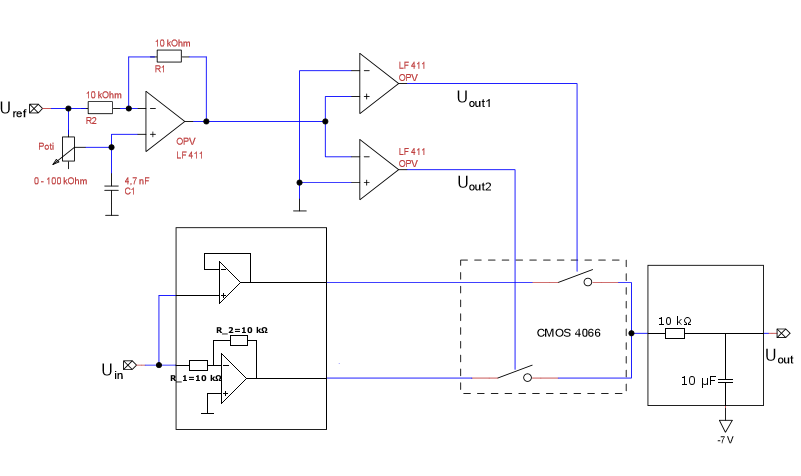
\includegraphics[scale=0.5]{./img/schaltung/gesamt.png}
    \end{center}
    \end{figure}
\end{frame}
\begin{frame}
    \frametitle{}
    \framesubtitle{}
    \begin{figure}[H]
    \begin{center}
            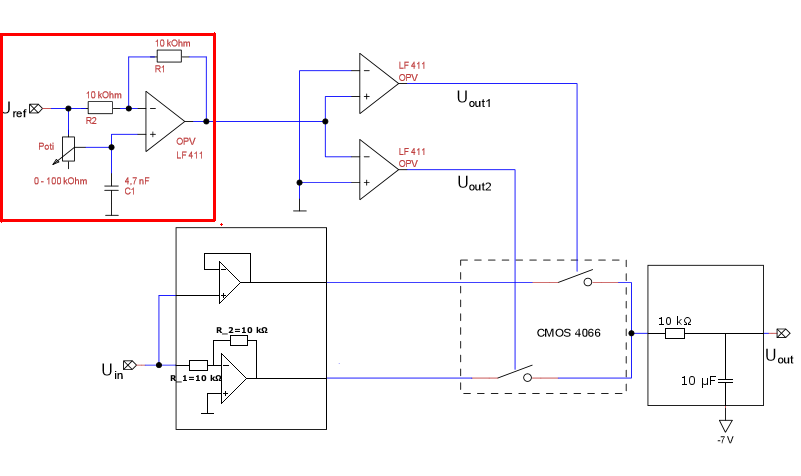
\includegraphics[scale=0.4]{./img/schaltung/gesamt_phase.png}
    \end{center}
    \end{figure}
    \begin{block}{}
        Phasenschieber bringt Referenzsignal auf Phase mit Messsignal
    \end{block}
\end{frame}
\begin{frame}
    \frametitle{}
    \framesubtitle{}
    \begin{figure}[H]
    \begin{center}
            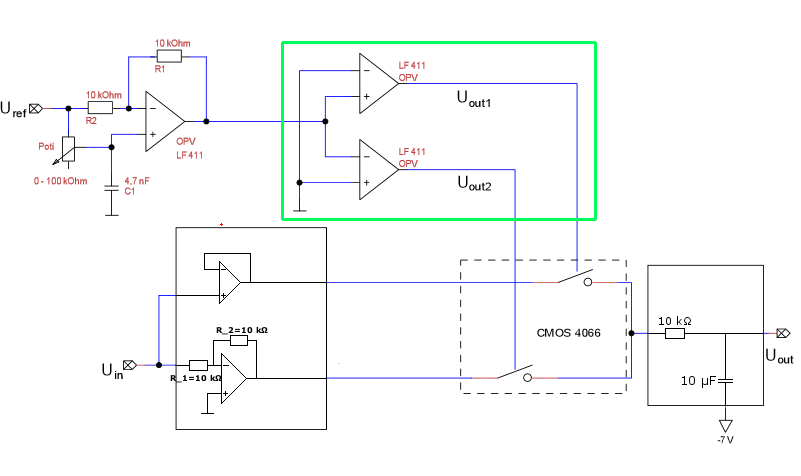
\includegraphics[scale=0.4]{./img/schaltung/gesamt_komp.png}
    \end{center}
    \end{figure}
    \begin{block}{}
        Komparatoren modulieren Sinus-Referenzsignal zu (gegensätzlichen) Rechtecksspannungen 
    \end{block}
\end{frame}
\begin{frame}
    \frametitle{}
    \framesubtitle{}
    \begin{figure}[H]
    \begin{center}
            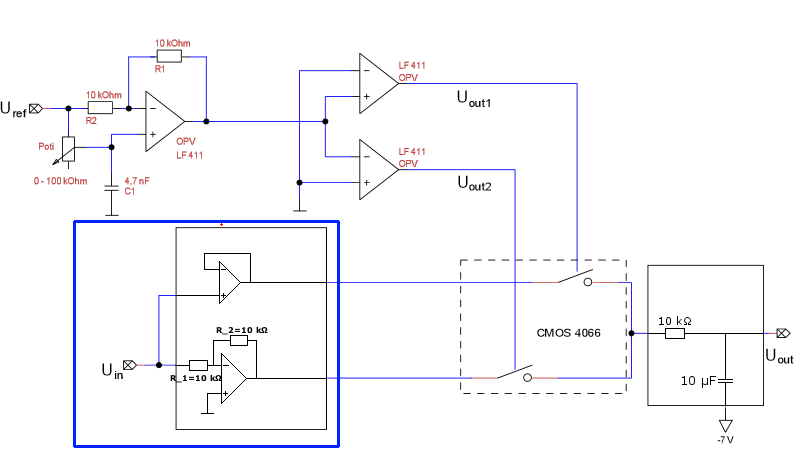
\includegraphics[scale=0.4]{./img/schaltung/gesamt_eing.png}
    \end{center}
    \end{figure}
    \begin{block}{}
        Eingangsverstärker lassen Signal durch und "drehen es um"
    \end{block}
\end{frame}
\begin{frame}
    \frametitle{}
    \framesubtitle{}
    \begin{figure}[H]
    \begin{center}
            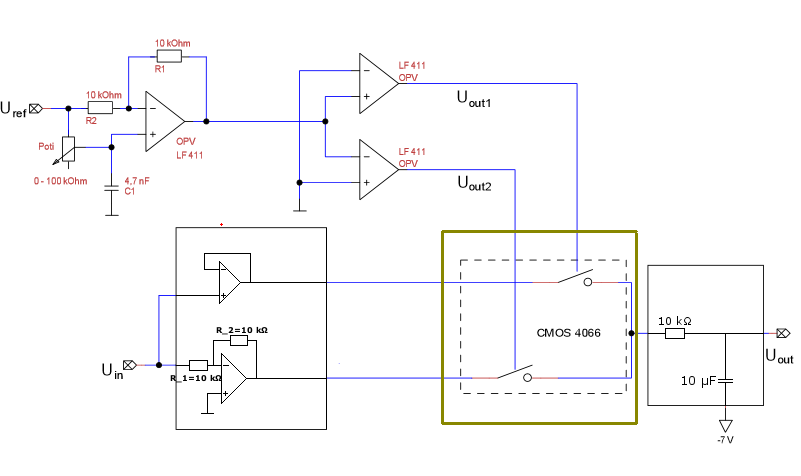
\includegraphics[scale=0.4]{./img/schaltung/gesamt_analog.png}
    \end{center}
    \end{figure}
    \begin{block}{}
        Analogschalter multipliziert Referenzsignale mit Messignalen
    \end{block}
\end{frame}
\begin{frame}
    \frametitle{}
    \framesubtitle{}
    \begin{figure}[H]
    \begin{center}
            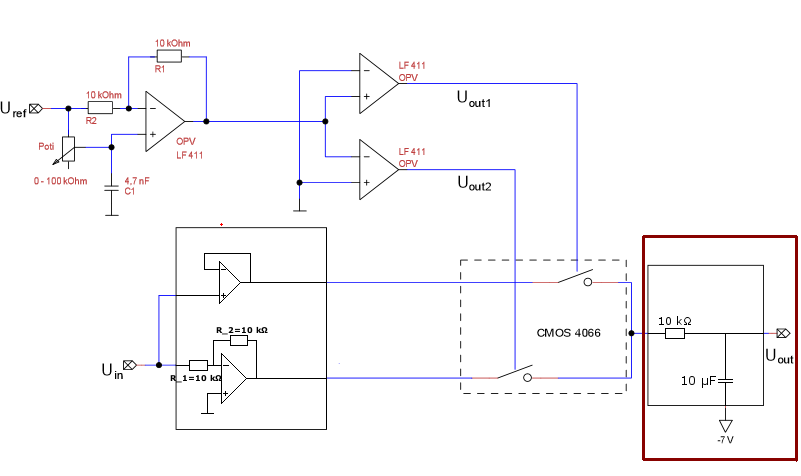
\includegraphics[scale=0.4]{./img/schaltung/gesamt_filter.png}
    \end{center}
    \end{figure}
    \begin{block}{}
        Tiefpassfilter integriert unerwünschte Frequenzen heraus
    \end{block}
\end{frame}
% subsection Ziel des Versuchs: (end)
% section Einführung (end)
